\documentclass{beamer}

\usepackage{graphicx,hyperref,udesc,url}
%\usepackage[latin1]{inputenc}
%\usepackage[T1]{fontenc}
\usepackage{listings}
\usepackage{booktabs}
\usepackage{bussproofs}
\usepackage{mathtools}
\usepackage[brazil]{babel}   
\usepackage[utf8]{inputenc}

\DeclarePairedDelimiter\ket{\lvert}{\rangle}

\title[Mini-Introdução à Teoria da Complexidade Quântica]{Mini-Introdução à\\ Teoria da Complexidade Quântica}

\author[Rafael Castro]{
    Rafael Castro\\\medskip
    {\small \url{rafaelcgs10@gmail.com}}}

\date{03 de Abril de 2019}

    \institute[UDESC]{
        Departamento de Ci\^encia da Computa\c{c}\~ao \\
            Centro de Ci\^encias e Tecnol\'ogicas\\
            Universidade do Estado de Santa Catarina}

\begin{document}

\begin{frame}
\titlepage

\end{frame}

\section{Fundamentos}

\begin{frame}
  \frametitle{Classe de Problemas na Computação Tradicional}
  \begin{itemize}
    \item NP: Problemas de decisão verificáveis em tempo polinomial.
    \item P: Problemas de decisão computáveis em tempo polinomial.

\end{frame}

\begin{frame}
\frametitle{Superposição}
\begin{itemize}
  \item A \textbf{Superposição quântica}: uma partícula pode assumir simultaneamente proporções entre dois estados.\\
  Ex: A polarização de um fóton pode ser qualquer proporção entre vertical ou horizontal. Mas uma vez que 
  observado, o seu estado colapsa (com base na probabilidade das proporções) para um dos extremos.
  \item A superposição quântica pode ser utilizada para representar informação binária: \textbf{qubit}.
  \item A computação quântica utiliza dados armazenados em qubits: 0 - 1 (qualquer proporção de ambos estados).
\end{itemize}
\end{frame}

\begin{frame}
\frametitle{Representação dos Qubits}
\begin{itemize}
  \item Os dois estados base de um qubit são representados pelos vetores

\begin{align}
\label{vet}
  \ket{0} \: = \begin{bmatrix} 
          1 \\ 
          0 \\ 
        \end{bmatrix}
  \:\text{e}\:
  \ket{1} \: = \begin{bmatrix} 
          0 \\ 
          1 \\ 
        \end{bmatrix}
\end{align}
Isso é conhecido como a notação de \textit{Dirac Ket} para vetores.
\item Para completamente representar o estado de um qubit são
  necessários dois números ($a, b$) \textbf{complexos} para descrever
  as duas proporções das duas bases:
\begin{align}
\label{amp}
  \Psi = a \ket{0} + b \ket{1}.
\end{align}
\end{itemize}
\end{frame}

\begin{frame}
\frametitle{Espaço de Estado de um Qubit}
\begin{itemize}
\item Utiliza-se a 2-norma:
  \begin{align}
    \label{sum1}
      |a|^2 + |b|^2 = 1
  \end{align}
\item O estado de um quibit pode ser visto como um valor com quatro graus de
liberdade. Devido a restrição da equação \ref{sum1} os possíveis valores de um
quibit se limitam uma equação de uma esfera de três dimensões.
\begin{figure}[h]
\label{bloch}
\centering
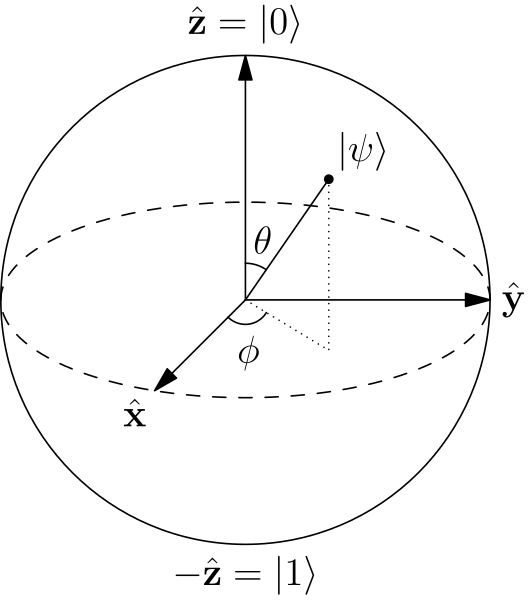
\includegraphics[width=0.25\textwidth]{bloch.png}
\caption{Esfera de Bloch. Fonte: Wikipedia.}
\end{figure}
\end{itemize}
\end{frame}

\begin{frame}
\frametitle{Operações em Qubits}
\begin{itemize}
  \item Operações em qubit são festas por produtos de matrizes unitárias, também chamado
  de transformação unitária.
  \item Uma transformação de um qubit é uma translação no espaço de estado.
  \item O qubit $\ket{0}$ está no polo norte da Esfera de Bloch é
    levado para o seu equador, um estado de superposição, pelo produto
    na Equação \ref{trans}.
       \begin{align}
         \label{trans}
       \begin{bmatrix} 
                 \frac{1}{\sqrt{2}} & \frac{1}{\sqrt{2}}\\ 
                 \frac{1}{\sqrt{2}} & -\frac{1}{\sqrt{2}}\\ 
       \end{bmatrix}
         \cdot
       \begin{bmatrix} 
                 1 \\ 
                 0 \\ 
       \end{bmatrix}
         =
       \begin{bmatrix} 
                \frac{1}{\sqrt{2}} \\ 
                \frac{1}{\sqrt{2}} \\ 
       \end{bmatrix}
       \end{align}
  \item Aplicar uma segunda vez essa transformação levaria novamente para o qubit $\ket{0}$.
\end{itemize}
\end{frame}

\begin{frame}
\frametitle{Emaranhamento Quântico}
\begin{itemize}
  \item Um par (ou mais) de partículas tem o seu estado associados de
  maneira que não é possível descrever o estado de uma delas
  individualmente.
  \item Por exemplo, dois \textit{spins} ($A$ e $B$) emaranhados por
seus campos magnéticos, ambos preparados no estado $\ket{0}$ e, então,
o \textit{spin} $A$ é colocado na superposição
$\frac{1}{\sqrt{2}} \ket{0} + \frac{1}{\sqrt{2}} \ket{1}$ por meio da
aplicação de um campo magnético oscilante. Se aplicado um outro campo
magnético no \textit{spin} $B$ que vai nega-lo (mudar para
$\ket{1}$) somente se o \textit{spin} $A$ estiver no estado $\ket{0}$,
então o \textit{spin} $B$ está nos estados $\ket{0}$ e $\ket{1}$ ao
mesmo tempo, devido ao emaranhamento com o \textit{spin} $A$. O sistema
final é uma superposição
$\frac{1}{\sqrt{2}} \ket{01} + \frac{1}{\sqrt{2}} \ket{10}$.
\end{itemize}
\end{frame}

\section{Computabilidade}

\begin{frame}
\frametitle{Portas Quânticas 1}
\begin{itemize}
  \item Portas quânticas são análogas as portas lógicas binárias: operam
    em $n$ bits/qubits e dão algum bit/qubit de resposta.
  \item Portas quânticas não perdem informação: são reversíveis.
  \item Considera a porta AND clássica e a porta quântica C-NOT (Control-NOT):
    \begin{figure}[!htb]
    \label{andcnot}
    \begin{minipage}{.4\textwidth}
      \centering
      \begin{tabular}{|l l|ll|}
      \hline
      A & B & A & $A$ AND $B$  \\ \hline
      0 & 0 & 0 & 0            \\ \hline
      0 & 1 & 0 & 0            \\ \hline
      1 & 0 & 1 & 0            \\ \hline
      1 & 1 & 1 & 1            \\ \hline
      \end{tabular}
    \end{minipage}
    \begin{minipage}{0.4\textwidth}
      \centering
      \centering
      \begin{tabular}{|l l|ll|}
      \hline
      A & B & A & $A$ CNOT $B$ \\ \hline
      0 & 0 & 0 & 0            \\ \hline
      0 & 1 & 0 & 1            \\ \hline
      1 & 0 & 1 & 1            \\ \hline
      1 & 1 & 1 & 0            \\ \hline
      \end{tabular}
    \end{minipage}
      \caption{Portas AND e CNOT.}
    \end{figure}
\end{itemize}
\end{frame}

\begin{frame}
\frametitle{Portas Quânticas 2}
\begin{itemize}
  \item Portas lógicas quânticas de $n$ qubits são transformações unitárias
    representadas por matrizes de tamanho $2^n \times 2^n$. Por exemplo,
    a porta lógica quântica CNOT tem a matriz unitária da Equação
    \ref{macnot} e a matriz da Equação \ref{trans} é a porta quântica
    Hadamard (H).
    \begin{align}
      \label{macnot}
    \begin{bmatrix} 
    1 & 0 & 0 & 0 \\
    0 & 1 & 0 & 0 \\
    0 & 0 & 0 & 1 \\
    0 & 0 & 0 & 1
    \end{bmatrix}
    \end{align}
\end{itemize}
\end{frame}

\begin{frame}
\frametitle{Circuitos Quânticos 1}
\begin{itemize}
  \item Circuitos (clássicos e quânticos) são um modelo de computação.
  \item Um circuito quântico é uma sequência de portas lógicas quânticas que
    operam sobre uma entrada de $n$ qubits.
  \item  \cite{be:97} provou que Circuitos Quânticos (com as devidas restrições)
    representam um modelo Turing-Completo.
  \item Não é trivial simular primitivas simples como
    \textit{looping}, \textit{branching} e composição no contexto de
    Máquinas de Turing Quânticas, pois as leis da Mecânica Quântica
    impõem restrições difíceis, como observar uma informação implica
    no colapso do seu estado.
\end{itemize}
\end{frame}

\begin{frame}
\frametitle{Circuitos Quânticos 2}
\begin{itemize}
  \item Portas Pauli-X/Y/Z, a raiz quadrada do NOT, a família de portas
    \textit{phase shift}, a porta \textit{swap} e porta Toffoli.
  \item Toffoli funciona de maneira simular à CNOT: atua em três bits
    e aplica o NOT no terceiro se, e somente se, os dois primeiros são
    um.
  \item Chama-se de \textit{conjunto universal de portas quânticas}
    (CUPQ) um conjunto portas quânticas capaz de construir circuitos
    que representam tudo que um computador quântico pode fazer.
  \item Foi demostrado por \cite{shi:03} que as portas Toffoli e
    Hadamard são um CUPQ.
  \item Foi demonstrado por \cite{da:06} que qualquer CUPQ pode
    ser simulado por outro CUPQ em tempo polinomial.
\end{itemize}
\end{frame}


\begin{frame}
\frametitle{Resultados de uma Computação Quântica}
\begin{itemize}
  \item Os resultados estão associados com
  uma probabilidade sobre a observação. Portanto, não é correto
  afirmar que algoritmos quânticos resolvem problemas da classe NP,
  \item Há diversas interpretações do que significa essa incerteza.
  \item Na Interpretação de Copenhagen os sistemas físicos tem
  propriedades não-determináveis (pois existem paralelamente) até
  serem observados (colapso da função de onda) e somente é possível
  afirmar probabilidades de resultados do ato de observar.
  \item A Interpretação de Muitos Mundos afirma que todos os possíveis
  resultados são objetivamente reais e o ato de observa (ou evento)
  cria novos ramos nas linhas temporais dos múltiplos universos e que
  as probabilidades dizem o quão provável é estar em algum desses
  vários mundos do ponto de vista observador.
\end{itemize}
\end{frame}

\section{Classes de Problemas}

\begin{frame}
\frametitle{Classe Probabilística BPP} 
\begin{itemize}
  \item A classe BPP (\textit{Bounded-Error Probabilistic
    Polynomial-Time}) são os problemas de decisão que podem ser
  resolvidos em tempo polinomial por uma Máquina de Turing
  Probabilística.
  \item Somente é aceitável no máximo $1/3$ de chance de fornecer a
  resposta errada (seja sim ou não).
  \item A classe BPP funciona como um análogo probabilístico da classe P.
  \item A verificação de primalidade de números é um exemplo de
    problema que estava na classe BPP, pois existem vários algoritmos
    probabilísticos como o bem conhecido Miller-Rabin. Porém,
    acabou-se encontrado um algoritmo determinista eficiente, logo
    passou a ser da classe P.
\end{itemize}
\end{frame}

\begin{frame}
\frametitle{Classe Quântica BQP} 
\begin{itemize}
  \item A classe de problemas resolvidos de maneira eficiente por
  computadores quânticos é a BQP (\textit{Bounded-Error Quantum
    Polynomial-Time}).
  \item Assim como a classe BPP, a classe BQP requer no máximo $1/3$ de
  chance de erro.
  \item Definida por Circuitos Quânticos.
  \item O número de qubits permitidos no circuito deve ser polinomial
    ao tamanho do problema, por exemplo algoritmo de Shor para
    fatoração de números primos de $n$-bits requer um circuito de
    $2n$-qubits.
\end{itemize}
\end{frame}


\begin{frame}
\frametitle{Relação Entre as Classes} 
\begin{itemize}
  \item BPP $\subseteq$ BQP, pois basta utilizar a porta Hadamard como
  um mecanismo de escolha probabilístico num qubit setado em
  $\ket{0}$.
  \item A classe PP é similar a BPP, mas com requisito de probabilidade
  difícil o suficiente para não ser possível aumentar a chance de
  acerto ao rodar o algoritmo várias vezes.
  \item A Classe PSPACE: problemas resolvidos com espaço polinomial,
  mas com tempo ilimitado.
  \item P $\subseteq$ BPP $\subseteq$ BQP $\subseteq$ PP $\subseteq$ PSPACE.
\end{itemize}
\end{frame}

\begin{frame}
\frametitle{O Maior Problema da Teoria da Complexidade Quântica} 
\begin{itemize}
  \item Computadores quânticos são fundamentalmente mais eficientes que
computadores probabilísticos clássicos? ou seja, se BPP $\not =$ BQP.
  \item A evidência mais popular que isso é verdade é o algoritmo
  quântico Shor e o fato que até hoje ninguém descobriu um eficiente
  algoritmo probabilístico que realiza o mesmo trabalho.
\end{itemize}
\end{frame}

\begin{frame}
\frametitle{BPP $\not \subseteq$ BQP por oráculo} 
\begin{itemize}
   \item A principal evidência, teórica, disso é o algoritmo de Simon
   \cite{si:94}.
   \item Suponha que exista uma função
   $f:\{0, 1\}^n \rightarrow \{0, 1\}^n$, a qual somente é possível
   acessar como um \textit{black box} (ou oráculo), apenas fornecendo
   entradas e olhando as saídas. O objetivo é descobrir uma
   mascara-XOR $s$, tal que para todos os pares distintos $(x, y)$
   tem-se que $f(x)=f(y)$ se, e somente se, $x \oplus y = s$ (aqui
   $\oplus$ é XOR bit a bit).
   \item Simon demonstrou, com o seu algoritmo, que um computador
   quântico resolve esse problema com no máximo $n$ perguntas ao
   \textit{black-box}, enquanto um computador clássico precisa de até
   $2^{n/2}$.
\end{itemize}
\end{frame}

\begin{frame}
\frametitle{Classes com Oráculos} 
\begin{itemize}
  \item Não há relação direta entre a classe NP e
  as classe probabilística BQP.
  \item Ao menos, sabe-se que a classe BPP está contida na classe
  NP$^{\text{NP}}$ (NP com um oráculo NP).
  \item Há a classe PH (Polynomial Hierarchy) que contém todos as
  classes com tempo polinomial estendidas com máquinas oráculos,
  inclusive NP e (curiosamente) BPP.
  \item O papel do oráculo é funcionar como uma espécie de
  medida de dificuldade do problema, quanto mais um algoritmo precisa
  consultar o oráculo, mais difícil é o problema.
  \item PH é uma generalização da classe NP, pois caso P = NP, então PH
  engloba todos os problemas de decisão que podem ser resolvidos em
  tempo polinomial por um computador clássico com acesso a um oráculo.
\end{itemize}
\end{frame}

\begin{frame}
\frametitle{BQP $\subseteq$ PH?} 
\begin{itemize}
  \item BQP está contida em PH?\\
   Isso questiona se há problemas somente tratáveis por um
   computador quântico, mesmo que P = NP
  \item Computadores quânticos são um caso a parte na Teoria da
   Complexidade?
  \item Em 2009 Aaronson introduziu o problema da ``fourrelação'' e
   demostrou estar em BQP \cite{aa:09}.
  \item Em Maio de 2018, os cientistas Ran Raz e Avishay Tal publicaram
   um artigo online \cite{ra:18} demonstrando que esse problema não
   está em PH.
  \item Uma computador quântico precisa de apenas uma consulta a um
   oráculo para resolver esse problema, enquanto um computador
   clássico não é capaz de resolve-lo de maneira eficiente, mesmo com
   um número ilimitado de consultas.
\end{itemize}
\end{frame}

\begin{frame}
  \frametitle{Ilha da Complexidade Quântica}
    \begin{figure}[h]
    \label{notph}
    \centering
    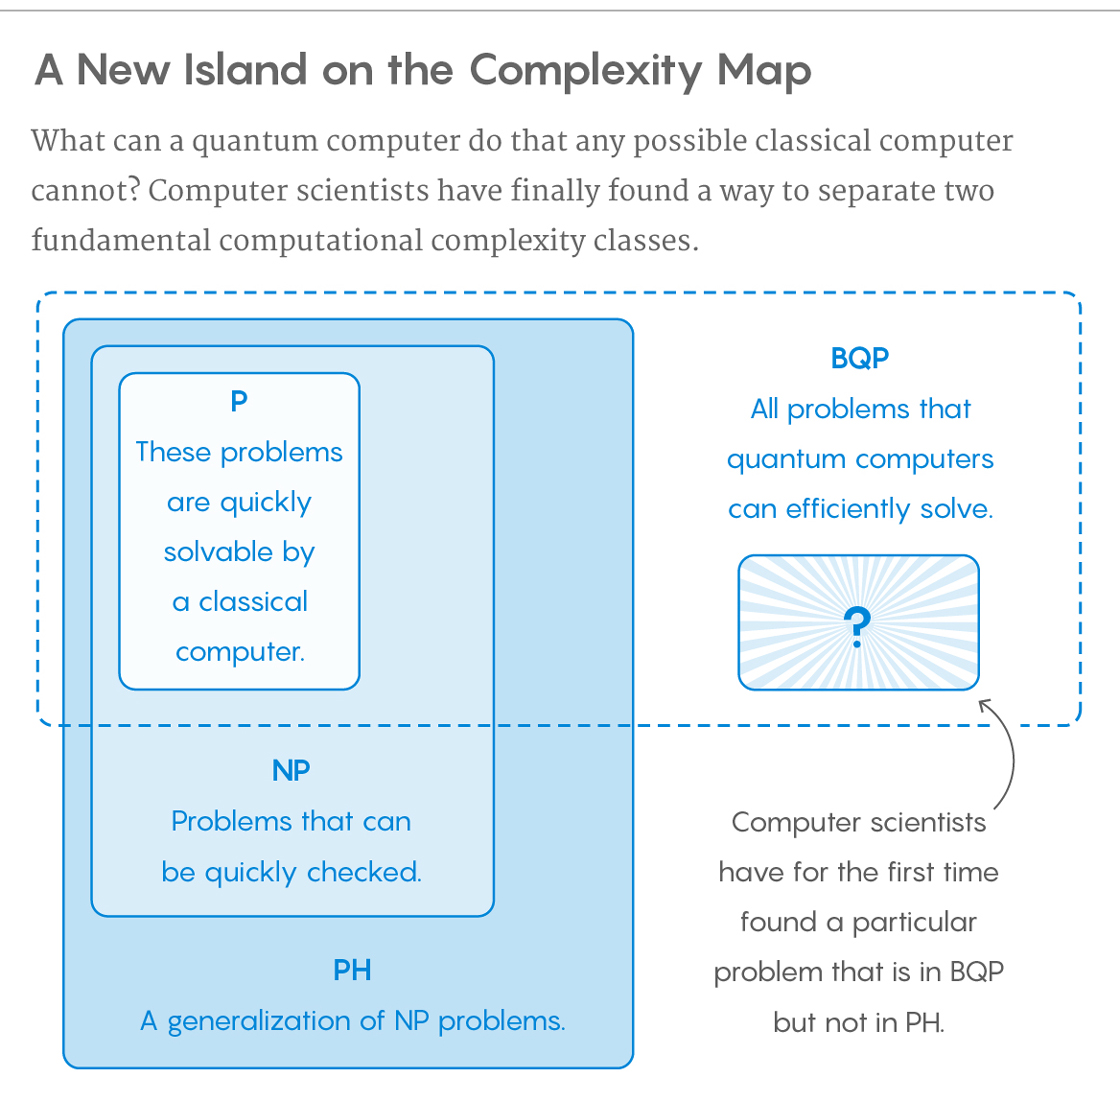
\includegraphics[width=0.6\textwidth]{island.jpg}
    \caption{Ilha de complexidade BQP. Fonte: QuantaMagazine.org.}
    \end{figure}
\end{frame}

\begin{frame}
\frametitle{\textit{Computational Complexity-Theoretic Church–Turing Thesis}} 
\begin{itemize}
  \item Esse novo resultado inválida a \textit{computational
    complexity-theoretic Church–Turing thesis}
  \item Proposto por \cite{be:97}, que diz que uma Máquina de Turing
  Probabilística pode simular em tempo polinomial qualquer outro
  modelo de computação.
  \item Algoritmos quânticos são eficientes em tarefas que
  algoritmos probabilísticos não são.
\end{itemize}
\end{frame}

\begin{frame}
\frametitle{NP-Completude e Computação Quântica} 
\begin{itemize}
  \item Erroneamente muitas pessoas ou sites/revistas de notícias
  anunciam que a computação quântica é capaz de resolver de maneira
  eficiente problemas NP-Completos.
  \item A ideia de que um computador quântico testa paralelamente todas
  as possibilidades e misteriosamente encontra a resposta é uma
  precipitação comum, ou seja, o status de NP $\subset$ BQP é
  desconhecido.
  \item Por outro lado, é sabido uma separação por oráculo de NP
  $\not \subset$ BQP: suponha um espaço de busca de tamanho $2^n$ de
  possíveis soluções e um oráculo que decide se a uma possível solução
  é a procurada.
  \item Num computador normal, no pior dos casos, é necessário $2^n$
  consultas no oráculo.
  \item Por meio do algoritmo de Groover \cite{gr:96} é possível
  encontrar a resposta em até $2^{n/2}$ consultas.
\end{itemize}
\end{frame}

\begin{frame}
\frametitle{Speed-up da Computação Quântica} 
\begin{itemize}
  \item O \textit{speed-up} da computação quântica para problemas de
  busca genéricos e não estruturados é quadrático. Não é conhecido
  como fazer \textit{speed-up} exponencial para esse tipo de problema.
  \item O motivo para o \textit{speed-up} ser quadrático é a 2-norma:
  \begin{itemize}
  \item Classicamente, num espaço de $N$ possíveis soluções com apenas
    uma correta (cada possibilidade com $1/N$ de ser a resposta), para
    um número $m$ de tentativas, tem a probabilidade de $m/N$ de
    adivinhar a solução. Assim, para ter uma boa chance de
    adivinhar a resposta correta é necessário ter um $m$ próximo a $N$.
  \item Já com a computação quântica é possível aplicar transformações
    lineares no vetor das amplitudes, que são as raízes quadradas das
    probabilidades por causa da 2-norma. Logo, para $m$ tentativas
    tem-se $m/\sqrt{N}$ de probabilidade de adivinhar a resposta. Com
    aproximadamente $\sqrt{N}$ tentativas a chance de encontrar a
    resposta já boa o suficiente.
  \end{itemize}
\end{itemize}
\end{frame}

\begin{frame}[allowframebreaks, noframenumbering]
  \frametitle{Referências}
   \bibliographystyle{apalike}
  \bibliography{sbc-template}
\end{frame}

\end{document}
%%% Local Variables:
%%% mode: latex
%%% TeX-master: t
%%% End:
